
%(BEGIN_QUESTION)
% Copyright 2006, Tony R. Kuphaldt, released under the Creative Commons Attribution License (v 1.0)
% This means you may do almost anything with this work of mine, so long as you give me proper credit

Qualitatively graph the response of an {\it integral-only} controller over time to the changes in process variable shown here:

$$\includegraphics[width=15.5cm]{i01599x01.eps}$$

Assume {\it direct} control action.

\vskip 20pt \vbox{\hrule \hbox{\strut \vrule{} {\bf Suggestions for Socratic discussion} \vrule} \hrule}

\begin{itemize}
\item{} Identify a fool-proof way to plot the curved output value of an integral controller as it ``sees'' a ramping PV or SP {\it input} value.
\item{} Explain how the output trend would look different if the time period of the second error (where PV steps away from and then back to SP in square-wave fashion) were longer in duration.
\end{itemize}

\underbar{file i01599}
%(END_QUESTION)





%(BEGIN_ANSWER)

The controller output graph shown here is {\it qualitative} only.  Although drawn to scale (i.e. all changes in the output are properly scaled relative to each other), the scale itself is arbitrary and therefore may not match the scale of your sketch:

$$\includegraphics[width=15.5cm]{i01599x02.eps}$$

%(END_ANSWER)





%(BEGIN_NOTES)

$$\includegraphics[width=15.5cm]{i01599x03.eps}$$

The output rate-of-change increases with increasing error between PV and SP, resulting in the downward-curving output response from point A to point B.  When the PV levels off between points B and C, the output rate-of-change remains steady, tracing a line going down at the same rate (slope) the curve terminated at point B.  Between points C and D the PV returns back to SP until the error is zero, causing the output to level off as its slope goes to zero.  

Between points D and E, the output holds its position because there is no error between PV and SP between those points of time.  When a sudden ``step change'' in PV occurs at point E, the output integrates at a constant rate upwards, then levels off when the PV returns to equal the SP.

%INDEX% Control, integral: graphing controller response

%(END_NOTES)


